\documentclass{article}
\usepackage[utf8]{inputenc}
\usepackage{url}
\usepackage{hyperref}
\usepackage{graphicx}

\title{Emotion challenge fact sheet}
\author{iCV}
\date{March 2020}

\begin{document}

\maketitle

\section{Team details}

\begin{itemize}
\item Team name
DeepBlueAI

\item Team leader name

Zhipeng, Luo
\item Team leader address, phone number and email

Address: No.27 Zhongguancun Road, Haidian District, Beijing 100190, China \\
Phone: 86-13051510090 \\
Email: luozp@deepblueai.com

\item Rest of the team members

Zhiguang,Zhang (equal contribution)

\item Team website URL (if any)

\item Affiliation
DeepBlue Technology

\end{itemize}

\section{Contribution details}

\begin{itemize}

\item Final score

It is not available now.

\item General method description

\begin{figure}
\centering
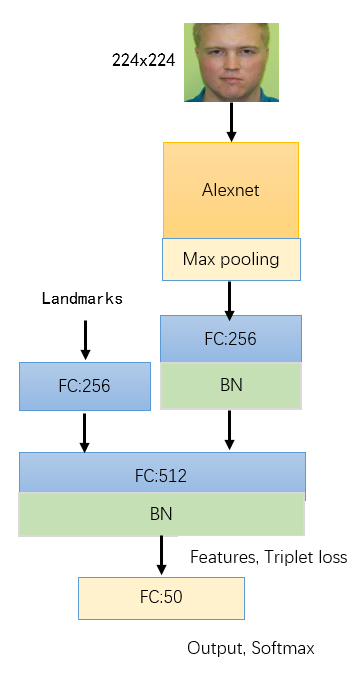
\includegraphics[width=4cm]{Net.PNG}
\caption{Architecture of the network architecture}
\label{fig:architecture}
\end{figure}

We fisrt extract the each ID's lamdmark feature, then calculate the difference between each landmark and the landmark of nose, then subsract each ID's mean as the geometrical information, then we get each ID's landmark offset of $R^{136\times1}$. And we use an modified AlexNet to extract the $R^{256\times1}$ feature of the $224\times224$ image on the second-last full connected layer. Then we concact the two features, and connect to a full connected layer. We use Triplt Loss and cross-entropy loss to train the net, the ground truth is a single label indicating the complementary and dominant emotion.

\item References

[1] Krizhevsky, Alex, Ilya Sutskever, and Geoffrey E. Hinton. "ImageNet classification with deep convolutional neural networks." neural information processing systems (2012): 1097-1105.

[2] Kazemi, Vahid, and Josephine Sullivan. "One millisecond face alignment with an ensemble of regression trees." Proceedings of the IEEE Conference on Computer Vision and Pattern Recognition. 2014.

[3] Iiris Lusi, Julio C S Jacques Junior, Jelena Gorbova, Xavier Bar,Sergio Escalera, Hasan Demirel, Juri Allik, Cagri Ozcinar, and Gholamreza Anbarjafari. Joint challenge on dominant and complementary emotion recognition using micro emotion features and head-pose estimation: Databases. In Automatic Face and Gesture Recognition, 2017. Proceedings. 12th IEEE International Conference on. IEEE,2017.

[4] J. Guo et al., ‘‘Multi-modality network with visual and geometrical information for micro emotion recognition,’’ in Proc. 12th IEEE Int. Conf. Autom. Face Gesture Recognit. (FG), May/Jun. 2017, pp. 814-819.

\item Describe data preprocessing techniques applied (if any)

Face detection and face landmark extraction using dlib and face crop and weakly aligned using the eyes center and the upper flip. We crop the image to 224x224 size.

\end{itemize}


\section{Face Landmarks Detection}
\subsection{Features / Data representation}
Describe features used or data representation model FOR FACE LANDMARKS DETECTION (if any)

\subsection{Dimensionality reduction}
Dimensionality reduction technique applied FOR FACE LANDMARKS DETECTION (if any)

\subsection{Compositional model}
Compositional model used, i.e. pictorial structure FOR FACE LANDMARKS DETECTION (if any)

\subsection{Learning strategy}
Learning strategy applied FOR FACE LANDMARKS DETECTION (if any)

\subsection{Other techniques}
Other technique/strategy used not included in previous items FOR FACE LANDMARKS DETECTION (if any)

\subsection{Method complexity}
Method complexity FOR FACE LANDMARKS DETECTION


\section{Dominant emotion recognition}
\subsection{Features / Data representation}
Describe features used or data representation model FOR DOMINANT EMOTION RECOGNITION (if any)

\subsection{Dimensionality reduction}
Dimensionality reduction technique applied FOR DOMINANT EMOTION RECOGNITION (if any)

\subsection{Compositional model}
Compositional model used, i.e. pictorial structure FOR DOMINANT EMOTION RECOGNITION (if any)

\subsection{Learning strategy}
Learning strategy applied FOR DOMINANT EMOTION RECOGNITION (if any)

\subsection{Other techniques}
Other technique/strategy used not included in previous items FOR DOMINANT EMOTION RECOGNITION (if any)

\subsection{Method complexity}
Method complexity FOR DOMINANT EMOTION RECOGNITION


\section{Complementary emotion recognition}
\subsection{Features / Data representation}
Describe features used or data representation model FOR COMPLEMENTARY EMOTION RECOGNITION (if any)

\subsection{Dimensionality reduction}
Dimensionality reduction technique applied FOR COMPLEMENTARY EMOTION RECOGNITION (if any)

\subsection{Compositional model}
Compositional model used, i.e. pictorial structure FOR COMPLEMENTARY EMOTION RECOGNITION (if any)

\subsection{Learning strategy}
Learning strategy applied FOR COMPLEMENTARY EMOTION RECOGNITION (if any)

\subsection{Other techniques}
Other technique/strategy used not included in previous items FOR COMPLEMENTARY EMOTION RECOGNITION (if any)

\subsection{Method complexity}
Method complexity FOR COMPLEMENTARY EMOTION RECOGNITION


\section{Joint dominant and complementary emotion recognition}
\subsection{Features / Data representation}
Describe features used or data representation model FOR JOINT DOMINANT AND COMPLEMENTARY EMOTION RECOGNITION (if any)

Landmark offset and AlextNet feature extraction.
\subsection{Dimensionality reduction}
Dimensionality reduction technique applied FOR JOINT DOMINANT AND COMPLEMENTARY EMOTION RECOGNITION (if any)

\subsection{Compositional model}
Compositional model used, i.e. pictorial structure FOR JOINT DOMINANT AND COMPLEMENTARY EMOTION RECOGNITION (if any)

\subsection{Learning strategy}
Learning strategy applied FOR JOINT DOMINANT AND COMPLEMENTARY EMOTION RECOGNITION (if any)

\subsection{Other techniques}
Other technique/strategy used not included in previous items FOR JOINT DOMINANT AND COMPLEMENTARY EMOTION RECOGNITION (if any)

\subsection{Method complexity}
Method complexity FOR JOINT DOMINANT AND COMPLEMENTARY EMOTION RECOGNITION


\section{Global Method Description}

\begin{itemize}
\item Total method complexity: all stages
\item Which pre-trained or external methods have been used (for any stage, if any)
\item Which additional data has been used in addition to the provided training and validation data (at any stage, if any)
\item Qualitative advantages of the proposed solution

If takes advantage of the geometry feature and texture pattern.
\item Results of the comparison to other approaches (if any)
\item Novelty degree of the solution and if is has been previously published
\end{itemize}

\section{Other details}

\begin{itemize}
\item Language and implementation details (including platform, memory, parallelization requirements)

We use Python with OpenCV and Dlib package and Pytorch deep learning framework.
\item Detailed list of prerequisites for compilation
\item Human effort required for implementation, training and validation?
\item Training/testing expended time?

Training takes about an hour on V100 GPU, test takes about half minute.
\item General comments and impressions of the challenge?

The task is hard, very prone to overfitting, and it's hard to find effective texture feature to do this challenge well.

\end{itemize}
\end{document}
